\section{Introduction}
\label{sec:intro}

合成孔径雷达（SAR）为海上监测提供了重要的图像来源。船型分类在目标检测的基础上，进一步识别已定位船只的类别。OpenSARShip、FUSAR-Ship等公开资源推动了学习式分类方法的研究与评价\cite{huang2018opensarship,hou2020fusar}。然而，实际应用要求分类器识别训练数据所覆盖条件之外的船只观测。本文关注已定位船舶图像切片（chip）上的这一问题：船型是需要识别的属性，而船舶所处的观测条件与场景可能发生变化。

同一艘船的重复观测直观体现了这一困难。图\ref{fig:observations}展示了不同成像批次下、关联到相同船舶身份的VV/VH图像。散货船在巴生港和理查兹湾的观测呈现出不同的方向及强响应空间排列；成品油/化学品船在同一港口、同一Sentinel-1A平台的两次观测中也存在外观变化，说明这种变化并不局限于跨港口或跨平台；原油轮在洛杉矶的两次观测同样表现出目标响应及周围结构的差异。尽管船舶身份与类别保持一致，其可见图像证据并非固定不变。这些自然观测为分析跨场景识别中的类内变化提供了直观起点。


\begin{figure*}[!t]
\centering
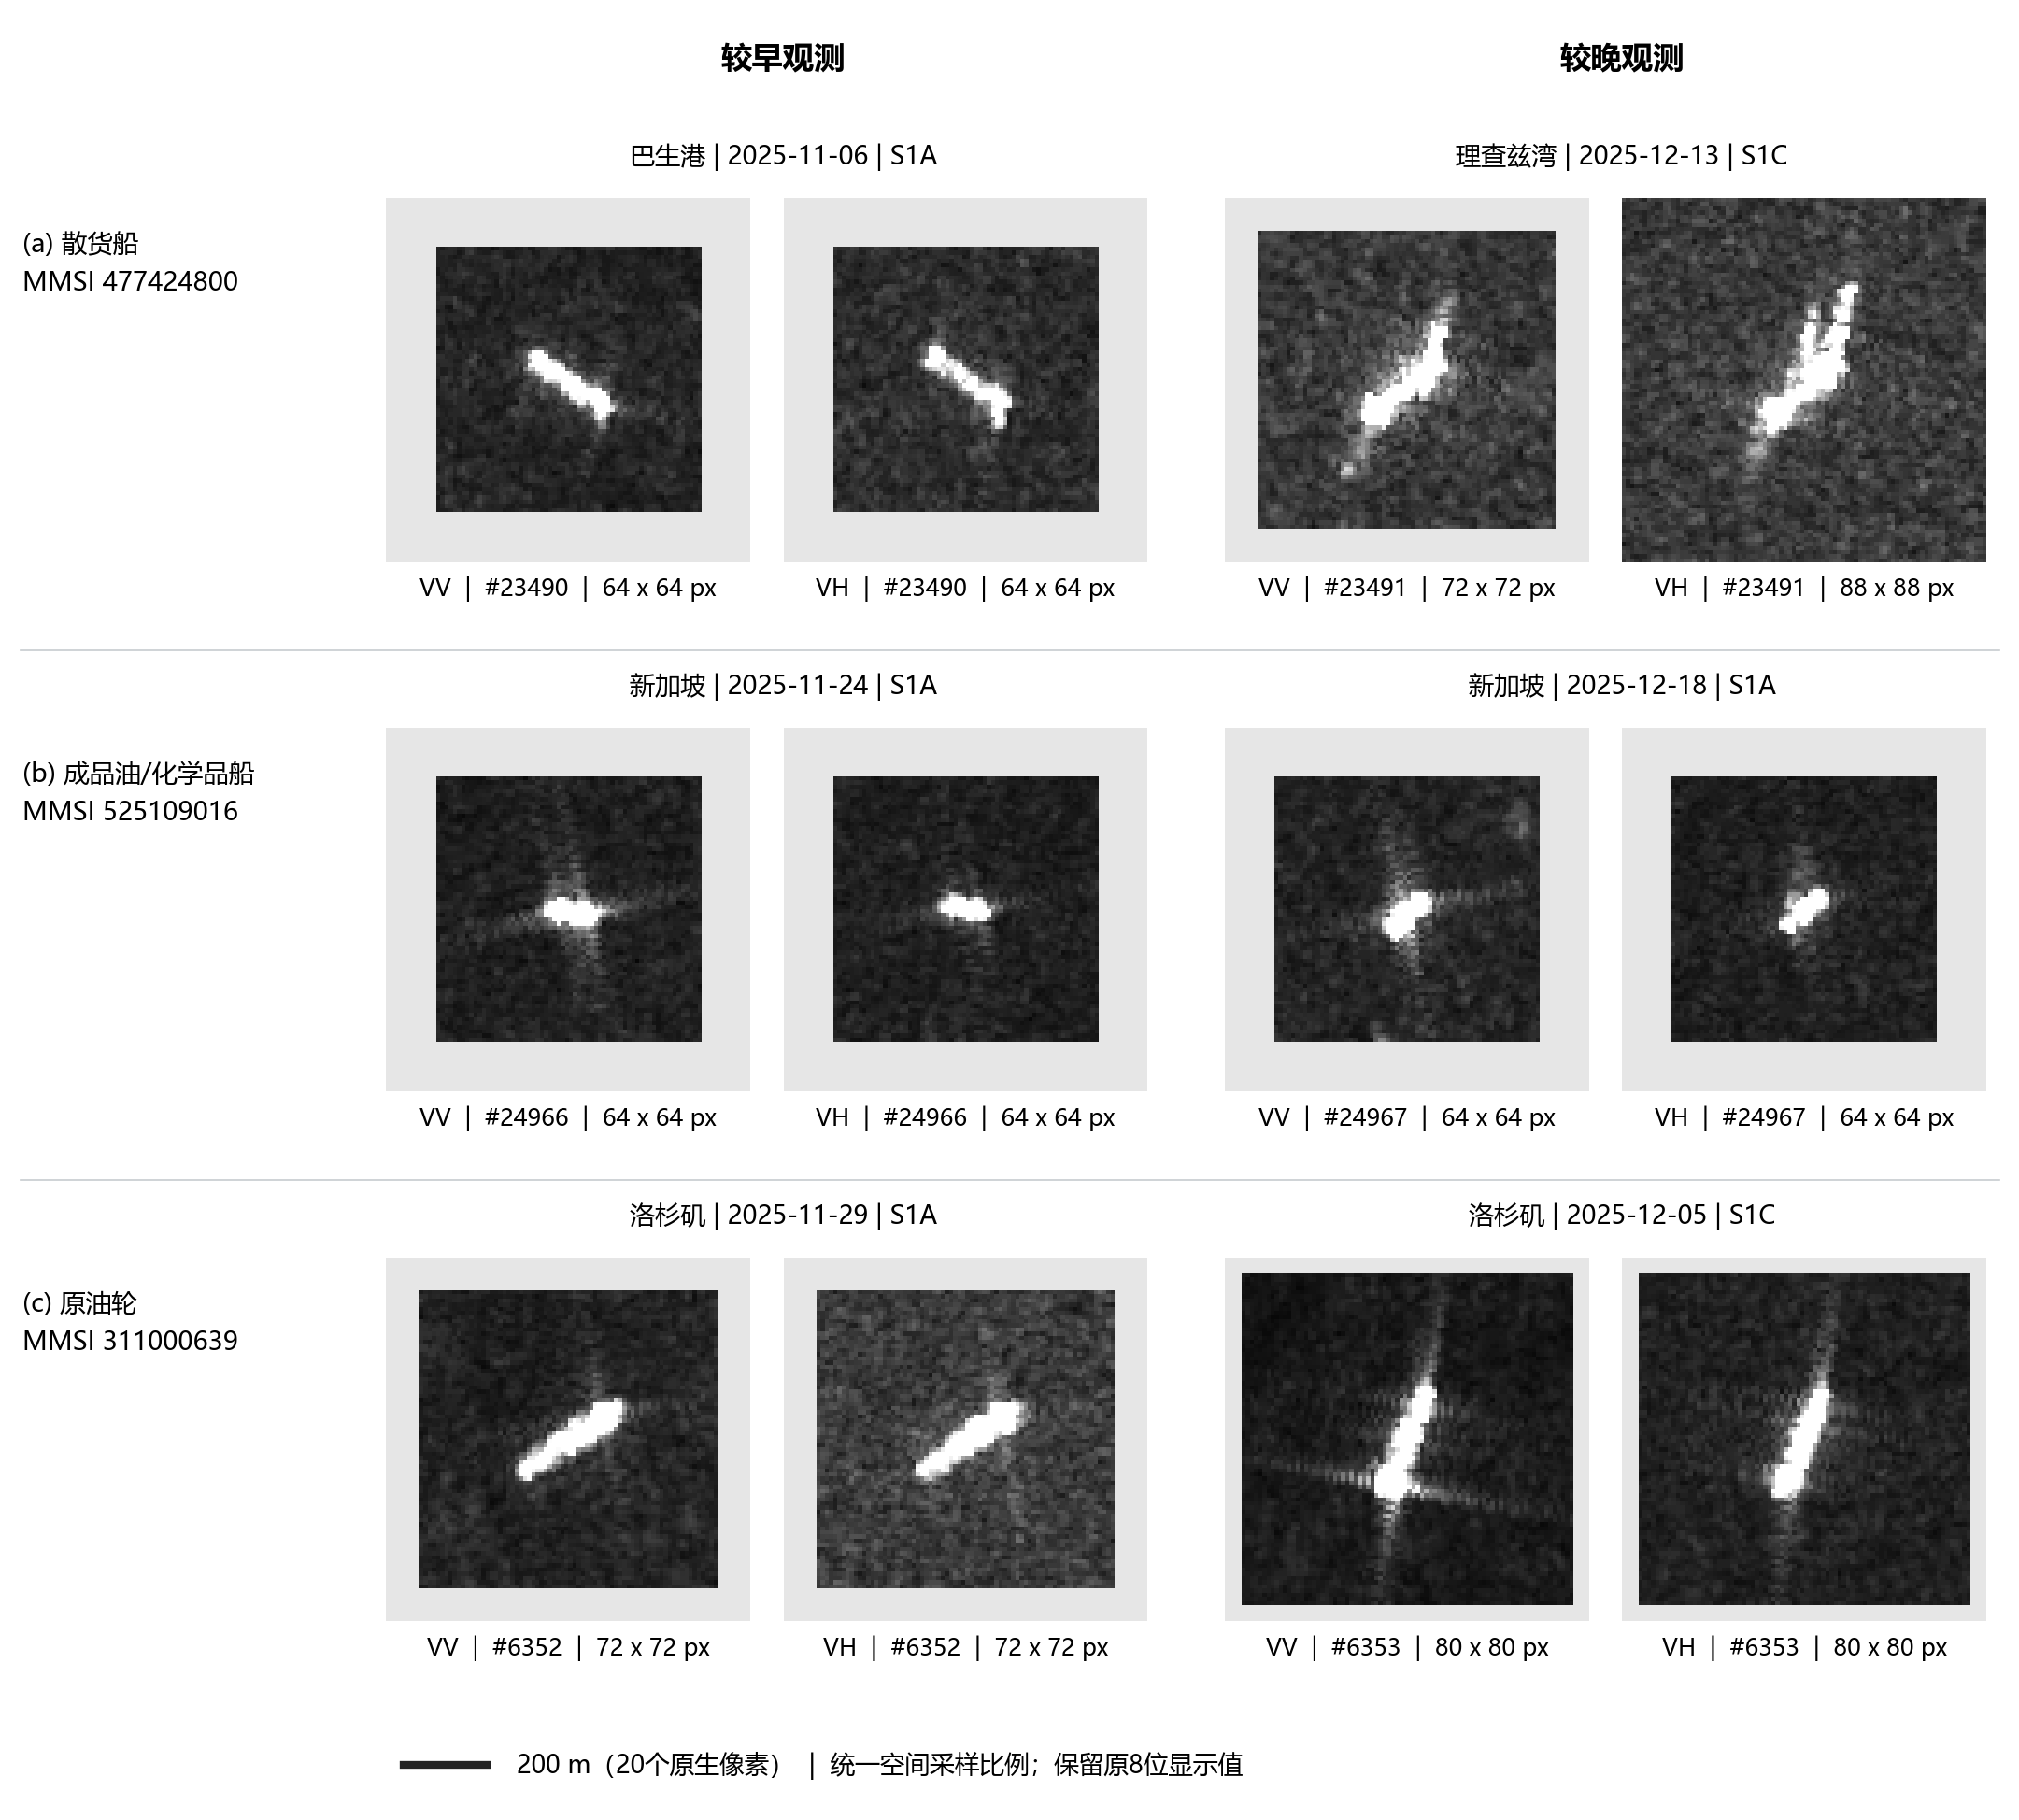
\includegraphics[width=\textwidth]{fig1_same_vessel_observation_shift.png}
\caption{24港数据中三艘船的配对观测：（a）不同港口、不同Sentinel-1平台的散货船；（b）相同港口、相同平台的成品油/化学品船；（c）相同港口、不同平台的原油轮。每行的船舶身份由相同MMSI关联，类别标签保持一致。较早、较晚观测分别展示VV和VH。保留所有原始像素，各面板按10 m/像素的共同空间采样比例显示，灰度范围固定为0–255；采样间隔不等于传感器分辨率。浅灰色表示原chip之外的留白，不属于图像。拼图未施加旋转、对比度增强、去噪或船长归一化。输入是已有8位显示产品，不是定标后向散射的定量比较。案例用于说明现象，不代表随机样本，也未单独隔离港口、几何或平台效应。}
\label{fig:observations}
\end{figure*}

相应的学习问题不只是如何缩小特征分布差异，还包括如何利用判别作用随条件而变化的图像证据。局部响应可能支持正确类别，也可能抬高竞争类别的分数，或者对最终决策影响很小。它的用途未必能仅由强度或空间位置决定。已有双极化船型分类方法通过共享特征提取、跨分支交互或高阶融合利用VV/VH的互补信息\cite{xie2023hogsiam,shao2023dpig,he2024cpinet}。在这些研究的基础上，本文进一步关注局部证据的来源与组织方式，以及这些证据在观测变化下如何影响类别竞争。

为研究这一问题，我们结合重复船舶观测与固定分类器上的受控扰动。自然配对在记录的船舶身份保持一致时，展示图像层面的变化；受控扰动则在其他输入与模型参数固定的条件下，改变指定极化、区域和空间尺度分量。后续问题分析部分的诊断实验表明，相近的局部操作在不同区域和极化中具有不同作用。同一操作在联合极化与单极化读出下，甚至可能产生方向相反的平均类别分差效应。判断改善有时来自竞争类别证据比正确类别证据下降得更多，而相近操作也可能破坏原有正确判断。这些结果刻画的是指定计算系统对受控输入变化的响应，并不等于识别了SAR采集过程中的独立物理原因。

由此，我们将研究问题聚焦为：\textbf{如何在保留局部响应的极化、区域与尺度身份的同时，学习它们在当前判别关系中的用途？} 目标不是统一抑制变化较大的响应，也不是预先把外围区域视为有害信息，而是在保留潜在线索的前提下，区分有效类别证据与误导性的类别竞争。受控扰动可以用于分析模型依赖，但固定模型敏感性与重新学习后的信息价值是不同的问题\cite{fong2017meaningful,hooker2019roar}。因此，本文将问题的实证刻画与分类方法的有效性验证分开：第\ref{sec:related}节梳理相关研究，后续问题分析部分给出支持方法设计的观测与扰动证据，后续再通过匹配的训练与评价检验设计是否改善识别。
